%% ma: L12-B17-0005
%% lop: 12
%% chuong: 5
%% bai: 17
%% dang: 12.17.5
%% loai: DS
%% muc: [VD, VD, VD, VDC]
%% dap_an: "ĐSSĐ"
%% nguon: "(NBV)-ĐỀ SỐ 6-MỖI NGÀY 1 ĐỀ THI 2025.pdf (D06, MỖI NGÀY 1 ĐỀ - Đề số 6), Phần II Câu 3 (THCS THPT Lê Thánh Tông - HCM 2025)"
%% kien_thuc: "Bài 14 (phương trình mặt phẳng, mặt phẳng trung trực), Bài 15 (phương trình tham số của đường thẳng), Bài 17 (mặt cầu); Bài 8 (độ dài vectơ); tiếp tuyến của mặt cầu (hình học phẳng)"
%% trang_thai: chinh-thuc
%% ghi_chu: "Giáo viên đã duyệt 10/10/2026. Đáp án gốc Đ S S Đ đúng (kiểm bằng sympy): a) 3449 km; b) 11315 km; c) 21425 km; d) va chạm tại H(6;5;6) sau 3 giờ. Lời giải gốc ý a) có lỗi in 4600 thay vì 6400 (kết quả 3449 vẫn đúng). Hình dựng lại: mặt cắt qua O chứa đường thẳng MN, tỉ lệ đúng (khoảng cách từ O đến MN là √97 ≈ 9,85); bỏ các điểm minh họa A, B, P, Q trên hình gốc"
\begin{ex}
Các thiên thạch có đường kính lớn hơn $140$ m và có thể lại gần Trái Đất ở khoảng cách nhỏ hơn $7\,500\,000$ km được coi là những vật thể có khả năng va chạm gây nguy hiểm cho Trái Đất. Để theo dõi những thiên thạch này, các nhà nghiên cứu của trung tâm Vũ Trụ Nasa đã thiết lập các trạm quan sát các vật thể bay gần Trái Đất. Giả sử có một hệ thống có khả năng theo dõi các vật thể ở độ cao không quá $4600$ km so với mực nước biển. Coi Trái Đất là khối cầu có bán kính $6400$ km. Chọn hệ trục tọa độ $Oxyz$ trong không gian có gốc $O$ là tâm Trái Đất và đơn vị độ dài mỗi trục là $1000$ km. Một thiên thạch (coi như một hạt) chuyển động với vận tốc $v_1=2\sqrt2\cdot10^3$ (km/h) không đổi theo đường thẳng xuất phát từ điểm $M(0;5;12)$ đến $N(12;5;0)$.
\begin{center}
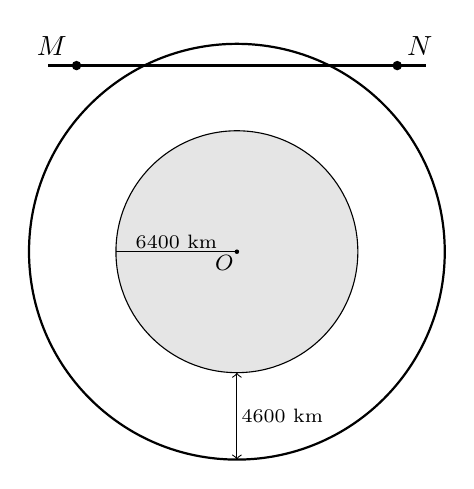
\begin{tikzpicture}[scale=.24]
  \def\R{11}\def\r{6.4}\def\h{9.849}\def\w{8.485}
  \draw[thick] (0,0) circle (\R);
  \draw[fill=gray!20] (0,0) circle (\r);
  \fill (0,0) circle (.12);
  \path (0,0) node[below left,font=\footnotesize,inner sep=1pt]{$O$};
  \draw[thick] (-\w-1.5,\h)--(\w+1.5,\h);
  \fill (-\w,\h) circle (.25) (\w,\h) circle (.25);
  \path (-\w,\h) node[above left]{$M$} (\w,\h) node[above right]{$N$};
  \draw[<->] (0,-\R) -- (0,-\r) node[midway,right,font=\scriptsize,inner sep=1.5pt]{$4600$ km};
  \draw (0,0)--(-\r,0) node[midway,above,font=\scriptsize,inner sep=1pt]{$6400$ km};
\end{tikzpicture}
\end{center}
\choiceTF
{\True Khoảng cách gần nhất từ thiên thạch đến Trái Đất bằng $3449$ km (làm tròn đến hàng đơn vị).}
{Các nhà nghiên cứu của trung tâm Vũ Trụ Nasa giả thiết nếu lúc thiên thạch đang ở vị trí $M$ bất ngờ đổi hướng và lao xuống Trái Đất theo phương thẳng thì quãng đường dài nhất nó có thể va chạm với Trái Đất là $14490$ km (làm tròn đến hàng đơn vị).}
{Tại thời điểm thiên thạch đang ở vị trí $M$ thì có $2$ vệ tinh đang ở vị trí $A(-6;-5;-6)$, $B(7;-6;7)$ có vận tốc khác nhau di chuyển trong mặt phẳng trung trực của $MN$ và luôn cách Trái Đất với khoảng cố định. Khoảng cách xa nhất của $2$ vệ tinh có thể đạt là $18412$ km (làm tròn đến hàng đơn vị).}
{\True Nếu vệ tinh $A$ đi với vận tốc $v_2=\dfrac{\pi\sqrt{97}}3\cdot10^3$ (km/h) thì sẽ va chạm với thiên thạch.}
\loigiai{$\overrightarrow{MN}=(12;0;-12)=12(1;0;-1)$, nên $MN$: $x=12+t$, $y=5$, $z=-t$. Mặt phẳng $(P)$ qua $O$ vuông góc với $MN$ là $x-z=0$; $(P)$ cắt $MN$ tại $H$ ứng với $12+2t=0$, tức $t=-6$, $H(6;5;6)$. Vì $(P)\perp MN$ tại $H$ nên $OH=\sqrt{97}$ là khoảng cách từ $O$ đến $MN$ (đơn vị $1000$ km).

a) Thiên thạch gần Trái Đất nhất khi đi qua $H$: $d=1000\sqrt{97}-6400\approx3449$ km. Đúng.

b) Quãng đường dài nhất là độ dài tiếp tuyến $ME$ kẻ từ $M$ đến Trái Đất: $OM=\sqrt{0^2+5^2+12^2}=13$, $OE=6{,}4$ nên $ME=\sqrt{13^2-6{,}4^2}\approx11{,}315$, tức $11\,315$ km. Sai.

c) Mặt phẳng trung trực của $MN$ đi qua trung điểm $H(6;5;6)$ và vuông góc $MN$, chính là $(P)$: $x-z=0$. Cả $O$, $A$, $B$ đều thuộc $(P)$ (vì $-6-(-6)=0$ và $7-7=0$). Hai vệ tinh luôn cách $O$ một khoảng không đổi nên chuyển động trên các đường tròn tâm $O$ bán kính $OA=\sqrt{97}$ và $OB=\sqrt{134}$. Khoảng cách xa nhất là $OA+OB=\sqrt{97}+\sqrt{134}\approx21{,}425$, tức $21\,425$ km $\ne18\,412$ km. Sai.

d) $H$ thuộc $(P)$ và $OH=\sqrt{97}=OA$ nên $H$ nằm trên đường tròn quỹ đạo của $A$, đối xứng với $A$ qua $O$ vì $\overrightarrow{OH}=(6;5;6)=-\overrightarrow{OA}$. Thiên thạch đến $H$ sau $\dfrac{MH}{v_1}=\dfrac{6000\sqrt2}{2\sqrt2\cdot10^3}=3$ giờ. Vệ tinh $A$ đi từ $A$ đến $H$ được nửa vòng tròn, dài $1000\pi\sqrt{97}$ km, mất $\dfrac{1000\pi\sqrt{97}}{\pi\sqrt{97}\cdot10^3/3}=3$ giờ. Hai thời gian bằng nhau nên chúng va chạm tại $H$. Đúng.}
\end{ex}
